\documentclass[12pt]{article}
\usepackage{amsmath,amsfonts,amsthm}
\usepackage{enumerate}
\usepackage{graphicx}
\usepackage{float}
\usepackage{multirow}
\usepackage{booktabs}
\usepackage{placeins}
\usepackage[round]{natbib}
\usepackage{hyperref}

\renewcommand{\baselinestretch}{1}
\topmargin 0in \headheight 0.0in \textheight 9in \textwidth 6.5in
\oddsidemargin 0.1in \evensidemargin 0.1in

\graphicspath{{../results/figures}}

\bibliographystyle{plainnat}


\begin{document}

\title{Evaluating LASSO Performance in High-Dimensional Data: A Comparison Between Pixel and Frequency Domains}
\author{Siyang Ren, Nichole E. Carlson, William Lippitt, Yue Wang}
\date{}
\maketitle


\section*{Notes}

Everything surrounded by [] are my thoughts/questions/to-dos.



\section{Introduction}

Spatial correlations in image data can significantly influence the performance of predictive models. When using images as predictors or outcomes, the inherent correlations between neighboring pixels often lead to challenges such as multicollinearity and reduced computational efficiency. To address the challenges posed by spatial correlations in image data, this study investigates whether using the eigendecomposition of \( M C M \) and its eigenvectors can effectively reduce spatial dependencies and improve model efficiency. Here, \( M \) is the centering matrix, and \( C \) is the spatial weights matrix, which encodes the assumed spatial relationships between pixels. The eigenvectors derived from \( M C M \) are used to transform the data into what is referred to as the ``frequency space''. This terminology reflects the analogy to signal processing, where the transformation decomposes data into spatially independent components, akin to frequencies. By reducing pixel correlations, this transformation may improve the efficiency and predictive performanace compared to use raw image data in analyses.

To test this hypothesis, we perform data simulations under different sparsity assumptions and compare the performance of LASSO models fitted in the original pixel space versus the frequency space. The results aim to provide insight into whether such spatial transformations enhance feature selection and prediction accuracy in high-dimensional datasets.



\section{Methods}

When dealing with image data, it's reasonable to assume that nearby pixels could have similar values, indicating spatial autocorrelation. Whether we use images as predictors or as outcomes, pixel correlations can impact model performance by reducing computational efficiency and stability if left unaddressed. Here, we discuss this effect in two scenarios: using images as predictors and as outcomes.

\subsubsection*{Image data as the predictor}

Suppose we have a set of images registered to the same template, and we want to predict a scalar outcome \( y \) using these images \( x \), where each has \( p \) pixels. If each pixel serves as a predictor, we can express the model for each observation as:
\[
  y_i = x_{i \cdot} \beta + \epsilon_i
\]
where \( i \) is the observation index and \( j \) is the pixel index. Here, \( y_i \) is the outcome, \( x_{i \cdot} \) represents an image as a row vector with \( p \) pixels, \( \beta \) is a column vector of \( p \) coefficients, and \( \epsilon_i \) is the error term, following a normal distribution with mean 0 and constant variance across observations. With many correlated pixels as predictors, multicollinearity can be an issue.

\subsubsection*{Image data as the outcome}

If we instead treat the images as outcomes, with \( p \) predictors, the model can be written as:
\[
  y_{i \cdot} = x_{i \cdot} \beta + \epsilon_{i \cdot}
\]
where \( y_{i \cdot} \) is a \( 1 \times s \) vector representing an image, \( x_{i \cdot} \) is a \( 1 \times p \) vector representing \( p \) predictors, \( \beta \) is a \( p \times 1 \) vector [William, is \( \beta \) a vector or a matrix?], and \( \epsilon_{i \cdot} \) is a \( 1 \times s \) vector of errors, which follows a distribution \( \mathcal{N}(0, \Sigma) \) that accounts for the correlation between pixels. One key assumption here is that the covariance structure \( \Sigma \) is shared across images.

As in generalized estimating equations (GEE), choosing an optimal covariance structure \( \Sigma \) involves balancing representation detail with computational efficiency: a simpler structure allows faster computation but may capture less detail, while a more complex structure provides a better fit but increases computational demands.

No matter whether we use the image data as predictors or outcomes, we need to address the correlation between pixels. Two main approaches are available: performing dimension reduction (e.g., applying PCA and retaining the top principal components) or reducing the complexity of the covariance structure of the image. In this paper, we focus on the second approach. Just as we used eigendecomposition on the Laplacian matrix for graph signal processing, and use the eigenvectors to transform the signal into frequency domain, here we use a different matrix to reflect spatial adjacency, not the Laplacian matrix, but one commonly used by Eigenvector Spatial Filtering, and perform a similar eigendecomposition and transform the image into a frequency space. We will design a few simulations to show that, the projected predictors in the frequency space has more prediction power than in the pixel space since the spatial autocorrelation is significantly reduced, and also because of the way we design the spatial adjacency matrix, it allows more interpretability in the frequency space we constructed.


\subsection{Frequency Space}

In this subection, we firstly introduce Moran's Coefficient (MC), a common measure of spatial autocorrelation, and then introduce a specially constructed spatial adjacency matrix combination, \( M C M \), and then show how the eigenvectors calculated by eigendecomposition on \( M C M \) have good explanation in the perspectivity of Moran's Coefficient.

\subsubsection{Moran's Coefficient and Eigenvector Spatial Filtering}

When dealing with spatially correlated data, like an image where pixel correlations depend on their relative positions, Moran’s Coefficient (MC) is a widely used measure of spatial autocorrelation. Suppose a vector \( x = (x_1, \ldots, x_p)^T \) represents an image with \( p \) pixels, and the spatial relationship between each pair of pixels is represented by a matrix \( C \), where \( C_{ij} \) indicates the spatial connection between pixels \( i \) and \( j \) (with diagonal elements equal to zero). According to \citet{griffith2014spatial}, the MC can be computed as follows:
\[
M C(x) = \frac{p}{\sum_{i=1}^p \sum_{j=1}^p c_{ij}} \cdot \frac{\sum_{i=1}^p \left(x_i - \bar{x} \right) \left[ \sum_{j=1}^p c_{ij} \left( x_j - \bar{x} \right) \right]}{\sum_{i=1}^p \left( x_i - \bar{x} \right)^2}
\]

\paragraph{Write Moran's coefficient in the matrix form}

To express Moran's coefficient (MC) in matrix form, we begin by defining the centering matrix \( M = I - \frac{1 1^T}{p} \), where \( I \) is the identity matrix and \( 1 \) is a column vector of ones. This matrix \( M \) is used to center the vector \( x \), ensuring it has a mean of zero. Specifically, applying \( M \) to \( x \) results in \( [M x]_i = x_i - \bar{x} \).

{\bf Claim:} Suppose \( \vec{a} \) and \( \vec{c} \) are column vectors of length \( n \), and \( B \) is an \( n \times n \) matrix. Then the expression \( \vec{a}^T B \vec{c} \) can be written as:
\[
  \vec{a}^T B \vec{c} = \sum_i \sum_j a_i B_{ij} c_j
\]
\begin{proof}
  The product \( B \vec{c} \) results in a column vector of size \( n \), with each entry \( i \) being \( \sum_j B_{ij} c_j \). Then, by multiplying with \( \vec{a}^T \):
  \[
    \vec{a}^T B \vec{c} = \sum_i a_i \left( \sum_j B_{ij} c_j \right) = \sum_i \sum_j a_i B_{ij} c_j.
  \]
\end{proof}

Using this, we can express the terms in the MC in matrix form:
\[
  \vec{1}^T C \vec{1} = \sum_{i=1}^p \sum_{j=1}^p 1 \cdot c_{i j} \cdot 1 = \sum_{i=1}^p \sum_{j=1}^p c_{i j} 
\]
\begin{align*}
  (M x)^T C (M x) & = \sum_{i=1}^p \sum_{j=1}^p (x_i - \bar{x}) c_{ij} (x_{j} - \bar{x}) \\
                  & = \sum_{i=1}^p (x_i - \bar{x}) \left( \sum_{j=1}^p c_{ij} (x_j - \bar{x}) \right)
\end{align*}
\begin{align*}
  x^T M x & = x^T M M x \\
          & = x^T M^T M x \\
          & = (M x)^T (M x) \\
          & = \sum_i (x_i - \bar{x})^2
\end{align*}
Thus, MC can be expressed as:
\[
  M C(x) = \frac{p}{\vec{1}^T C \vec{1}} \cdot \frac{x^T M C M x}{x^T M x}
\]

The matrix form can further be reorganized as:
\[
  M C (x) = \frac{(M x)^T C (M x)}{\vec{1}^T C \vec{1}} / \frac{(M x)^T I (M x)}{\vec{1}^T I \vec{1}}
\]
where the numerator represents the covariance of \( x \) along the spatial structure \( C \), and the denominator represents the covariance of \( x \) assuming an independence structure \( I \) [I'm still unclear about the interpretation of ``covariance along a structure''].

[Regarding the expectation of \( M C \): I'm unclear on the distinction between ``the expected value when there is no correlation in the assumed model'' and ``the value when there is no correlation in the input.'' What does ``correlation'' refer to in each context? According to Wikipedia, the expectation of \( M C \) under the null hypothesis of no spatial autocorrelation is \( -1 / (n - 1) \), and I found a proof \href{https://stats.stackexchange.com/questions/567411/expectation-and-variance-of-morans-i-under-the-null}{here} which I don’t fully understand. In my understanding, no spatial autocorrelation means all elements of \( C \) equal zero (which seems to conflict with the \( -1 / (n - 1) \) expectation).]

\paragraph{Eigendecompose MCM and its key properties}

\citet{de1984extreme} demonstrated that, when \( C \) is symmetric, the maximum and minimum possible values of the Moran coefficient correspond to the largest and smallest eigenvalues of the matrix \( MCM \). Since the Moran coefficient for an eigenvector is a function of its corresponding eigenvalue (which we will prove later), the eigenvector associated with the largest eigenvalue of \( MCM \) yields the highest Moran coefficient. This indicates that this vector captures the strongest spatial autocorrelation among all vectors, given the spatial structure defined by \( C \).

{\bf Claim:} The centering matrix \( M \) is idempotent, meaning \( M^2 = M \).

\begin{proof}
  \begin{align*}
    M^2 = M M & = \left( I - \frac{1 1^T}{n} \right) \left( I - \frac{1 1^T}{n} \right) \\
              & = I - \frac{1 1^T}{n} - \frac{1 1^T}{n} + \frac{1 1^T 1 1^T}{n^2} \\
              & = I - \frac{2}{n} 1 1^T + \frac{n 1 1^T}{n^2} \\
              & = I - \frac{1 1^T}{n} = M
  \end{align*}
\end{proof}

We can now consider the eigendecomposition of \( M C M \), which can be written as:
\[
  M C M = E \Lambda E^{T}
\]
where \( \Lambda \) is a diagonal matrix of eigenvalues, and \( E \) contains the corresponding eigenvectors as columns. We define \( \lambda_i \) and \( v_i \) to be the \( i \)-th eigenvalue and eigenvector, respectively.

Since \( M C M \) is symmetric, the eigenvectors are orthogonal (i.e., \( E E^T = I \)). Additionally, the eigenvectors corresponding to non-zero eigenvalues are orthogonal to the vector of ones, \( E^T 1 = 0 \), because \( M C M 1 = 0 \).

Now, we prove that for any eigenvector \( v_i \), \( M v_i = v_i \).
\begin{proof}
  \begin{align*}
    M C M v_i & = \lambda_i v_i \\
    M^2 C M v_i & = \lambda_i M v_i \\
    M C M v_i & = \lambda_i M v_i \\
    \lambda_i v_i & = \lambda_i M v_i \\
  \end{align*}

  For \( \lambda_i \neq 0 \), this implies \( M v_i = v_i \).
\end{proof}

With this property established, we can show that the Moran coefficient for each eigenvector is proportional to its corresponding eigenvalue. The Moran coefficient for an eigenvector \( v_i \) is given by:
\[
  M C (v_i)=\frac{n}{1^T C 1} \frac{v_i^T M C M v_i}{v_i^T M v_i}.
\]

Using \( M C M v_i = \lambda_i v_i \) and \( M v_i = v_i \), this expression simplifies to:
\[
  M C (v_i)=\frac{n}{1^T C 1} \lambda_i.
\]

Thus, the Moran coefficient is directly proportional to the eigenvalue \( \lambda_i \), as required.

\subsubsection{Whitening Transformations}

We now explain how the properties we established about the Moran coefficient and the eigenvectors of \( M C M \) can be used to reduce data complexity when fitting image data into models.

A common approach to reducing covariance complexity is the whitening transformation, which transforms a vector of random variables (e.g., an image) to yield a diagonal covariance matrix, meaning no correlation between pixels [Note: strictly speaking, the whitening transformation yields an identity covariance matrix, not just diagonal, so ``whitening'' may not be the most accurate term here. Perhaps ``decorrelation transformation'' is more appropriate. For now, I'll use ``whitening'' for consistency]. Multiple whitening (decorrelation) transformations are possible, but orthogonal transformations are popular due to their preservation of vector length. [I understand that orthogonal transformations maintain vector length (image size) and can be thought of as a rotation/reflection, but it’s unclear why this property is advantageous.]

If we flatten a 2D image into a 1D column vector \( x \), an orthogonal transformation can be viewed as a rotation or reflection of this vector without changing its length.
\begin{proof}
  The length of \( x \) can be expressed as \( x^T x \). Applying an orthogonal matrix \( E \), which satisfies \( E E^T = I \), to \( x \), the length of the transformed vector \( E^T x \) is \( (E^T x)^T (E^T x) = x^T x \).
\end{proof}

A common way to find an orthogonal matrix is through eigen decomposition of a symmetric matrix, which provides a diagonal matrix of eigenvalues and an orthogonal matrix of eigenvectors. Here, we perform eigen decomposition on the centered adjacency matrix \( M C M \) as described earlier. This approach is particularly useful for transforming data with spatial autocorrelation due to its interpretability. In this case, the eigenvector associated with the \( n \)-th largest eigenvalue captures the \( n \)-th strongest spatial autocorrelation direction, as defined by \( C \). This orthogonal transformation can thus be viewed as rotating or reflecting the original data to align with these spatial directions [I'm trying to picture how an image would appear along the direction of strongest spatial autocorrelation]. Since this decomposition is not based on the actual covariance of the dataset, it may not fully eliminate pixel correlation. However, if the adjacency matrix \( C \) is well estimated, we expect the transformed data to have sufficiently reduced pixel correlations, improving computational efficiency.

The next question is how to select an appropriate adjacency matrix \( C \) for an image. For an image with \( s \) pixels, \( C \) will be an \( s \times s \) matrix, where each element \( C_{ij} \) represents the adjacency between pixels \( i \) and \( j \). There are several ways to define adjacency between pixels. 

One approach is data-independent and unweighted, where only 0 or 1 values are assigned in \( C \): 1 for adjacent pixels and 0 otherwise. A common example is the “2-neighbor adjacency matrix,” where two pixels are considered adjacent if they are direct neighbors or share a direct neighbor. All other values, including the diagonal, are set to 0.

Another approach is data-independent but weighted, assigning adjacency values based on the distance between two pixels. Suppose the distance between pixels \( i \) and \( j \) is \( d_{ij} \), calculated using their Euclidean distance in the image; then the adjacency \( C_{ij} = - \exp(d_{ij}) \). Both methods define adjacency based on relative pixel positions rather than their actual values.

After choosing an adjacency matrix \( C \), we can apply the eigendecomposition of \( M C M \) as we discussed above, and get the \( E \) contains the eigenvectors as columns. The eigenvector \( v_i \), corresponding to the \( i \)-th largest eigenvalue, represents the \( i \)-th strongest spatial autocorrelation that could be captured by a vector among all possible vectors. Suppose \( X \) represents a \( n \times p \) matrix, representing \( n \) images, with each row corresponding to one image follow the spatial adjacency we just specified. Transforming images \( X \) to the frequency space is achieved by projecting it onto the matrix of eigenvectors:
\[
  X_{\text{freq}} = X \cdot E
\]

Suppose \( X \) can be labeled into two classes, 0 and 1, decided by some pattern of it. The labels represented by a vector \( y \), with the probability of \( y_i = 1 \) decided by \( \eta_i = 1 / (1 + \exp(-X \cdot \vec{\beta})) \). Here \( \vec{\beta} \) is a coefficient vector of length \( p \), with values equals to a constant non-zero value \( \beta \), indicating the area deciding the label, and values equal to 0 for the other areas. Then to ensure each \( \eta \) remains the same before and after whitening transformation, the coefficient vector \( \vec{\beta} \) can be transformed into the coefficient vector in the frequency space, denoted by \( \vec{b} \).
\[
  X \cdot \vec{\beta} = X_{\text{freq}} \cdot \vec{b} = (X \cdot E) \cdot \vec{b} = X \cdot (E \cdot \vec{b})
\]
so \( \vec{\beta} = E \cdot \vec{b} \).


\subsection{Models}

\subsection{Simulations}

Our first simulation simulates the scenario that images are used as predictors for binary classification problem.

\subsection{Analyses}


Our simulation starts from simulating the scenario where we want to classify images into a binary class. Suppose \( X \) represents a \( 1000 \times 256 \) matrix of 1000 observed images, with each row corresponding to one image. The pixel values of each image was randomly generated from a multivariate normal distribution with zero mean and a \( 256 \times 256 \) covariance matrix \( C_{\text{cov}} = - \exp (\text{dist} (x_i, x_j)) \), where \( \text{dist} (x_i, x_j) \) represents the Euclidean distance between any two pixels \( i \) and \( j \) in an 2D image. The simulated image will then be flattened into a 1D sequence of length 256, with each pixel be used as a predictor in the model.

We are planning to simulate the scenario that the center \( 8 \times 8 \) area decides the classification results of an image, with larger values (meaning darker colors) be class 1, and others as class 0. To realize this, we define the coefficient vector \( \vec{\beta} \) to have value 0 in the positions corresponding to the surrounding area in an image, and value \( \beta \) in the positions corresponding to the center \( 8 \times 8 \) area in the image. The response vector \( y \), which will be a vector of 0 and 1, will be simulated from binomial distributions for each position independently. The success probability of \( y_i = 1 \) will be \( p_i = 1 / (1 + \exp (- X_{i \cdot} \vec{\beta})) \).

We then evaluate the ability of Logistic regression to identify the pixels that decide the classification of an image, in other words, the coefficients with non-zero values. A logistic regression with L1 penalty will be applied.

Then, we need to test whether the white transformation using the eigendecomposition results we just proposed could significantly reduce the correlation between predictors and thus improve the model performance. Since in practice we don't know the actual covariance matrix of \( X \), with the assumption that the covariance between two pixels are reflected in their spatial adjacency matrix, and the whitening transformation method we just proposed, we assume a spatial adjacency matrix \( C_{\text{adj}} \), which is in the format of:
\[
  C_{ij} = 
  \begin{cases}
    - \exp (\text{dist} (x_i, x_j))  & \quad x_i \neq x_j \\
    0                                & \quad x_i = x_j
  \end{cases}
\]
Note here we assume that the spatial adjacency matrix is identical to the actual covariance matrix (ignore the diagonal elements), and we will evaluate in the future the scenario that they are not identical.



Similarly, we will fit a Logistic regression model with L1 penalty with \( y \) on \( X_{\text{freq}} \) again, and compare the predicted coefficients with \( \vec{b} \).

The experiment above compares the performance of Logistic regression model with L1 penalty when the predictors are correlated with each other, and only a proportion of them are significant (in other words, there are sparsity in the coefficient vector \( \vec{\beta} \)), we next evaluate how the model performance by fitting with the predictors in the original space and frequency space when the coefficient vector in the frequency space is sparse (in other words, \( \vec{b} \) is sparse). This represents the scenario that the image is dominated by a few spatial patterns.





\subsection*{Model Evaluation}

To compare the performance of LASSO in both the pixel space and frequency space, we fit two models: one using covariates in the pixel space and another using covariates in the frequency space. The optimal regularization parameter \( \lambda \) is selected via cross-validation, using the binomial deviance as the performance metric. The dataset is split into training (80\%) and test (20\%) sets, and the cross-validation is performed using 10 folds.

Two values of \( \lambda \) are considered: 
\begin{itemize}
  \item \texttt{lambda.min}, which minimizes the cross-validated error.
  \item \texttt{lambda.1se}, the largest \( \lambda \) within one standard error of the minimum.
\end{itemize}

After selecting the optimal \( \lambda \), we evaluate model performance on the test set. The performance metrics include:
\begin{itemize}
  \item Accuracy
  \item Area Under the Curve (AUC)
  \item P-values for each covariate
\end{itemize}

P-values are computed using the \texttt{hdi} package [need to provide further details on how the package computes p-values]. The entire simulation is repeated 500 times. We report the mean and standard deviation of accuracy and AUC. For p-values, we report the percentage of cases where \( p < 0.05 \) at each covariate location [consider whether p-value adjustment is needed here].


\section*{Results}

\subsection*{Effect Size Determination}

In Simulation 1, we evaluated the distribution of the success probability \( \mathbf{p} \) at different non-zero values of \( \beta \) (0.01, 0.05, 0.1, 0.2, and 1). As shown in Figure \ref{fig:sim1_p_dist}, a value of 0.1 produced the most uniform distribution of \( \mathbf{p} \), making it the optimal choice for model fitting in this scenario.

Similarly, in Simulation 2, we assessed the distribution of \( \mathbf{p} \) at various non-zero values for \( \mathbf{b} \) (0.1, 0.15, 0.2, 0.25, and 0.3). As shown in Figure \ref{fig:sim2_p_dist}, the value of 0.2 resulted in the most uniform distribution of \( \mathbf{p} \), making it the best option for this simulation.

\begin{figure}[h!]
	\centering
	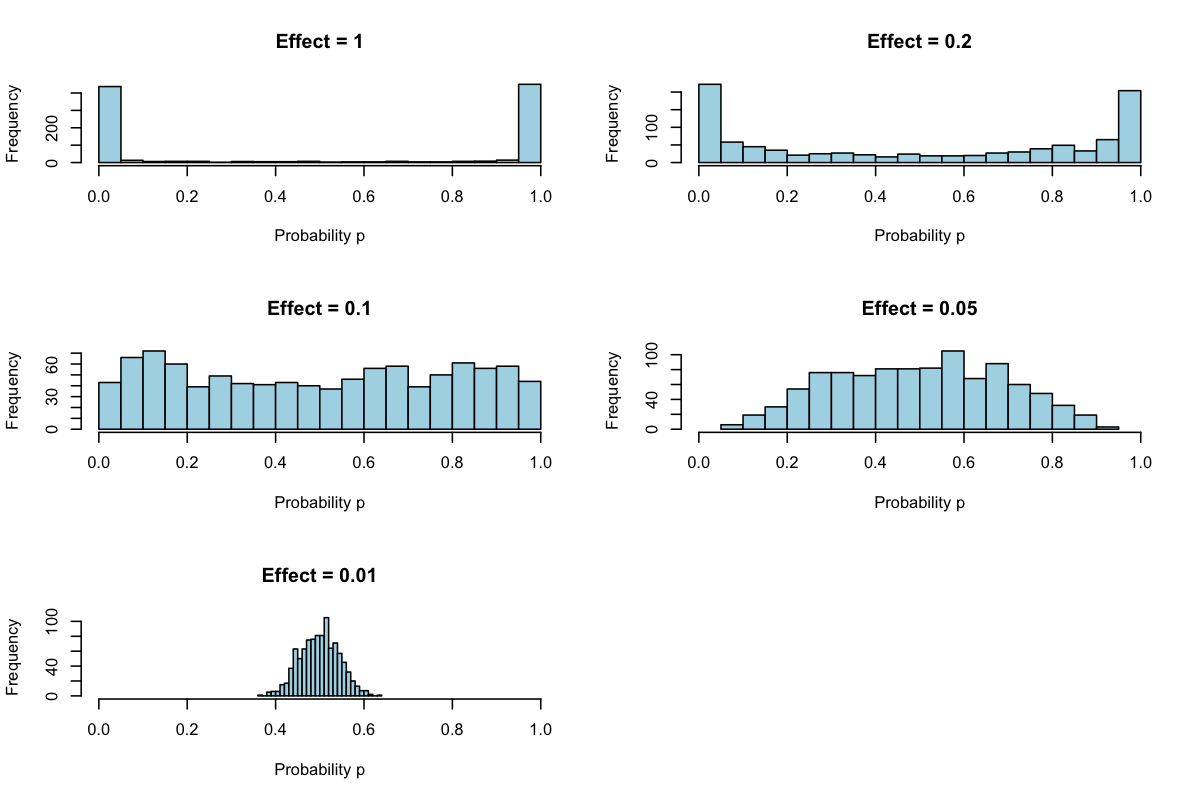
\includegraphics[width=0.8\textwidth]{sim1_p_dist.png}
  \caption{Distribution of success probability \( \mathbf{p} \) at different non-zero values in Simulation 1.}
	\label{fig:sim1_p_dist}
\end{figure}

\begin{figure}[h!]
	\centering
	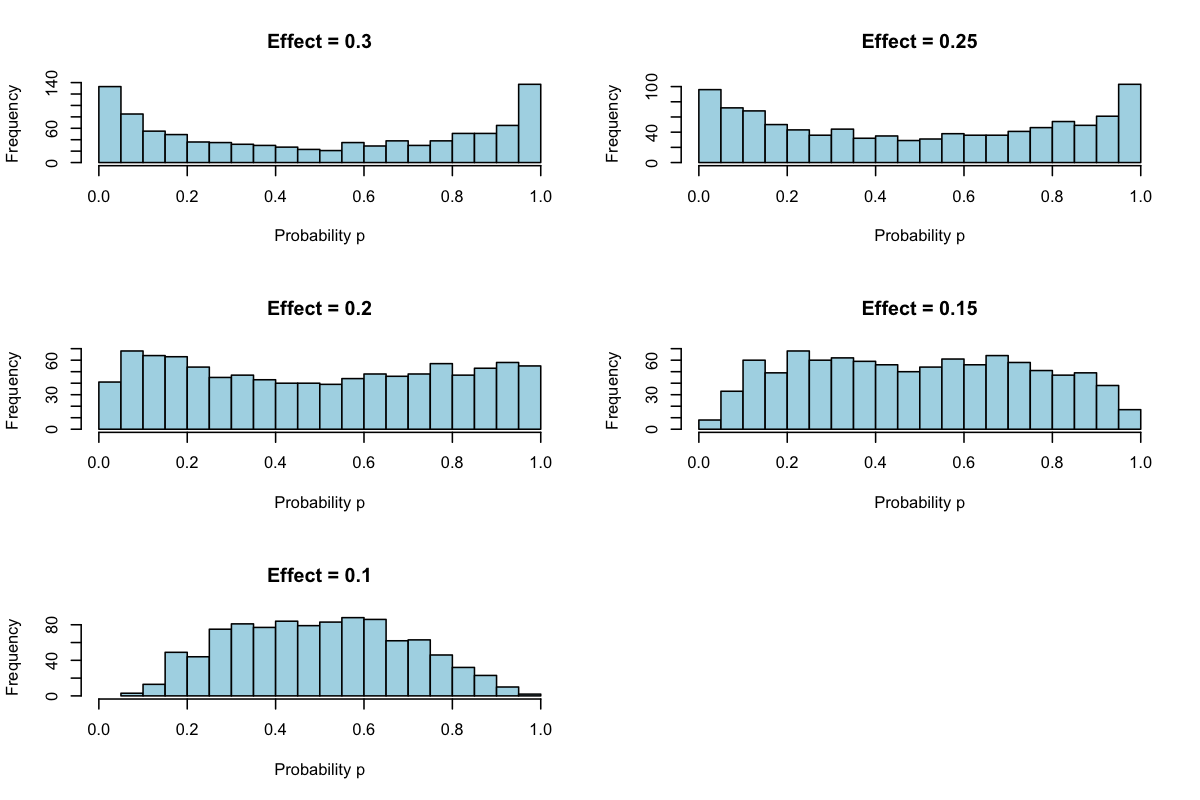
\includegraphics[width=0.8\textwidth]{sim2_p_dist.png}
  \caption{Distribution of success probability \( \mathbf{p} \) at different non-zero values in Simulation 2.}
	\label{fig:sim2_p_dist}
\end{figure}

\FloatBarrier

\subsection*{Group Mean Difference}

In this subsection, we examine the group mean differences in covariate values between instances where \( y = 1 \) and \( y = 0 \) for both Simulation 1 and Simulation 2.

Figure \ref{fig:group_diff1} presents the group mean differences for Simulation 1, with the heatmap on the left showing that regions corresponding to non-zero coefficients in \( \beta \) exhibit larger mean differences between \( y = 1 \) and \( y = 0 \), as larger covariate values in these locations have higher probabilities of being assigned to \( y = 1 \). The scatterplot on the right displays the group mean differences in the frequency domain, where each point represents a frequency component; frequencies associated with larger eigenvalues tend to have larger mean differences. Figure \ref{fig:coefs_sim1} shows the actual coefficients used in Simulation 1, where non-zero coefficients in \( \beta \) are localized to specific pixels, corresponding to the areas with larger mean differences in the group comparison.

\begin{figure}[h!]
	\centering
  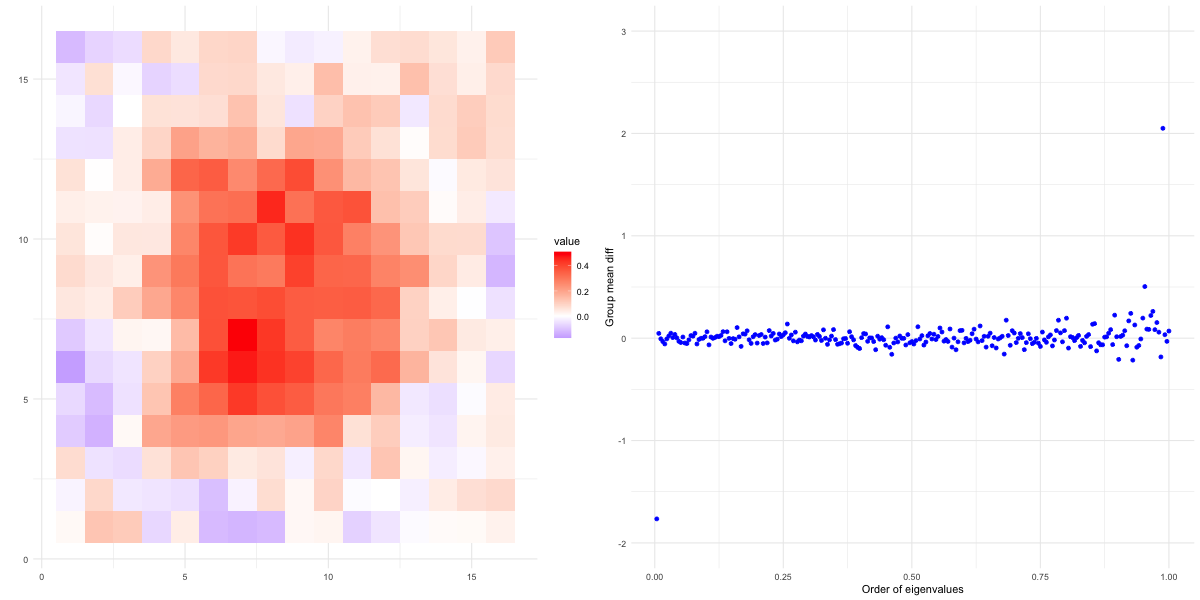
\includegraphics[width=0.8\textwidth, height=0.35\textwidth]{group_mean_diff_sim1.png}
	\caption{Group mean difference in covariate values between instances where \( y = 1 \) and \( y = 0 \) in Simulation
		1, shown for both the pixel space (left) and frequency space (right).}
	\label{fig:group_diff1}
\end{figure}

\begin{figure}[h!]
	\centering
	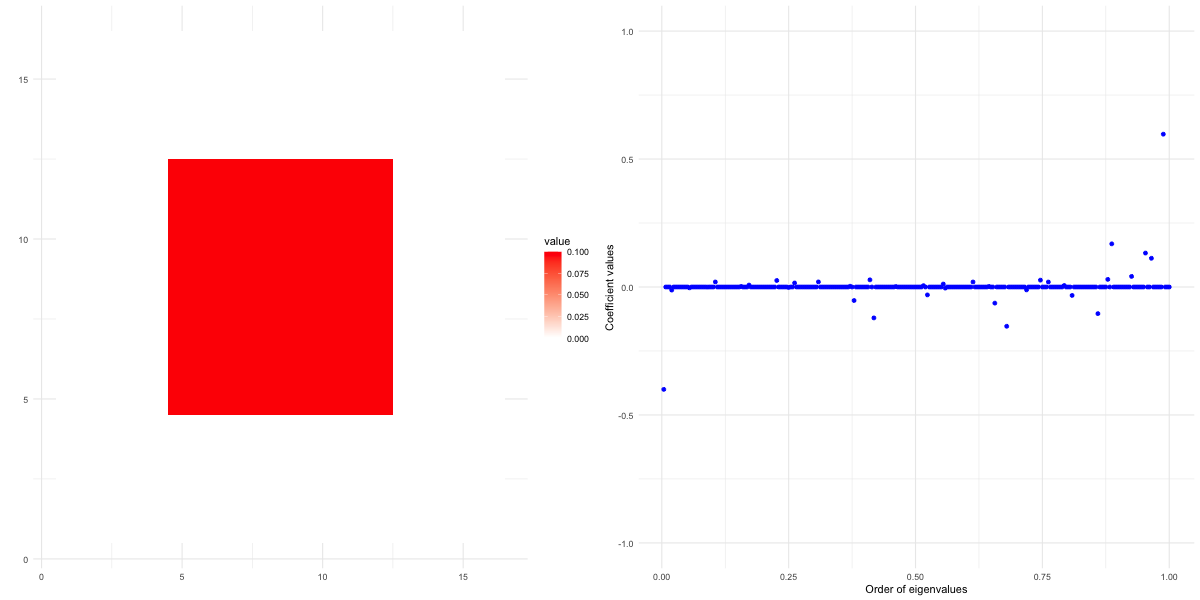
\includegraphics[width=0.8\textwidth, height=0.35\textwidth]{actual_coefs_sim1.png}
	\caption{Actual coefficients in Simulation 1 for the pixel space (left) and frequency space (right).}
	\label{fig:coefs_sim1}
\end{figure}

Figure \ref{fig:group_diff2} shows the group mean differences for Simulation 2, while Figure \ref{fig:coefs_sim2} displays the actual coefficients. The non-zero coefficients in \( \mathbf{b} \) are uniformly set to 0.2. However, the scatterplot in the frequency space does not clearly highlight the non-zero components, with increasing variance observed for larger eigenvalues. This variance pattern is consistent with the diagonal covariance matrix used in the simulation. The difficulty in identifying the non-zero components suggests that the effect size may be too small relative to the variance, making detection challenging. [Further adjustments to either the effect size or the covariance matrix could improve the detectability of these non-zero coefficients in future analyses.]

\begin{figure}[h!]
	\centering
	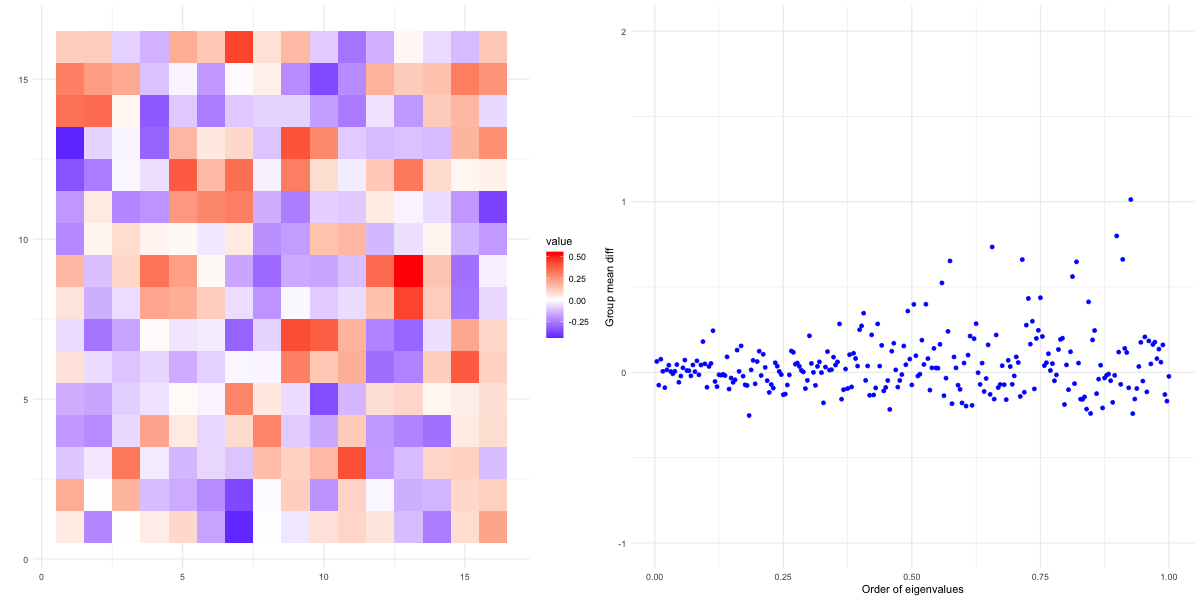
\includegraphics[width=0.8\textwidth, height=0.35\textwidth]{group_mean_diff_sim2.png}
	\caption{Group mean difference in covariate values between instances where \( y = 1 \) and \( y = 0 \) in Simulation 2.}
	\label{fig:group_diff2}
\end{figure}

\begin{figure}[h!]
	\centering
	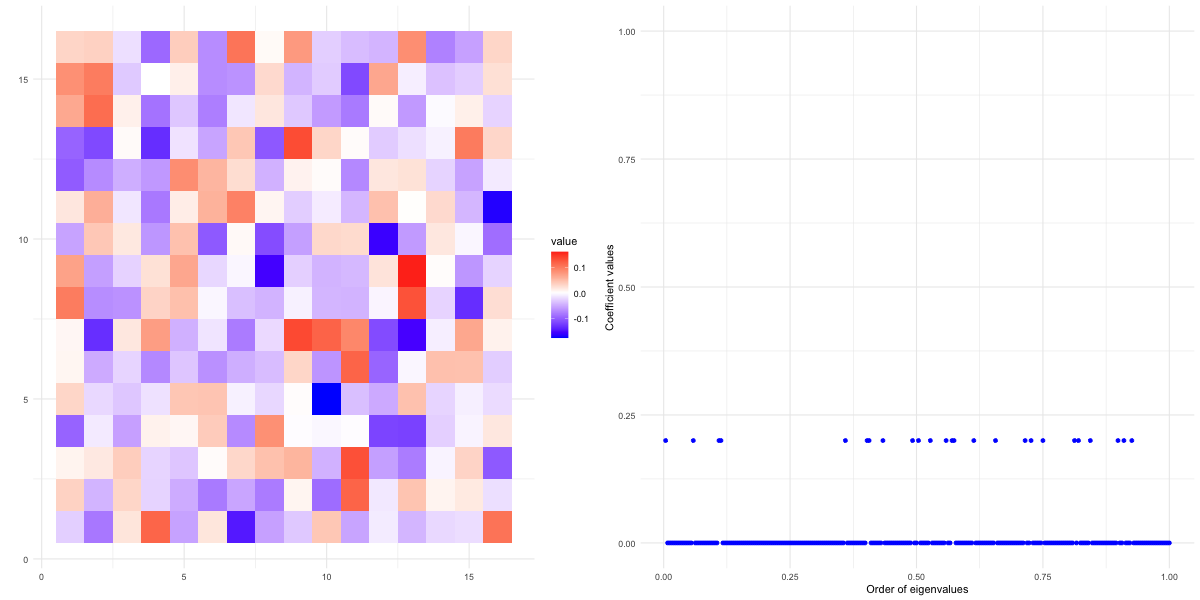
\includegraphics[width=0.8\textwidth, height=0.35\textwidth]{actual_coefs_sim2.png}
	\caption{Actual coefficients in Simulation 2 for the pixel space (left) and frequency space (right).}
	\label{fig:coefs_sim2}
\end{figure}

\FloatBarrier

\subsection*{AUC and Accuracy}

Table~\ref*{tab:auc_acc_table} summarizes the average AUCs and accuracies over 500 iterations. In both Simulation 1 (pixel space sparsity) and Simulation 2 (frequency space sparsity), models fitted in the frequency space consistently outperformed those fitted in the pixel space. For example, in Simulation 1, using \texttt{lambda.min} as the regularization parameter, models trained with pixel space covariates achieved an AUC of 0.803 (SE = 0.031) and an accuracy of 72.6\% (SE = 0.032). In contrast, models trained with frequency space covariates produced a slightly higher AUC of 0.826 (SE = 0.028) and a higher accuracy of 74.5\% (SE = 0.030). A similar trend was observed in Simulation 2, with frequency space models showing superior performance regardless of the regularization parameter used.

\begin{table}[h!]
	\centering
	\caption{Comparison of AUC and accuracy between models fitted in the pixel space and frequency space across 500 iterations for Simulation 1 and Simulation 2.}
	\label{tab:auc_acc_table}
	\begin{tabular}{l|cc|cc}
		\toprule
		\textbf{Simulation}   & \multicolumn{2}{c}{\textbf{Model in Pixel Space}} & \multicolumn{2}{c}{\textbf{Model in Frequency Space}}                                              \\
		\midrule
		                      & \textbf{AUC (SE)}                                 & \textbf{Accuracy (SE)}                                & \textbf{AUC (SE)} & \textbf{Accuracy (SE)} \\
		\midrule
		\textbf{Simulation 1} &                                                   &                                                       &                   &                        \\
    \texttt{lambda.min}            & 0.803 (0.031)                                     & 0.726 (0.032)                                         & 0.826 (0.028)     & 0.745 (0.030)          \\
      \texttt{lambda.1se}            & 0.800 (0.032)                                     & 0.722 (0.032)                                         & 0.826 (0.029)     & 0.745 (0.031)          \\
		\midrule
		\textbf{Simulation 2} &                                                   &                                                       &                   &                        \\
    \texttt{lambda.min}            & 0.755 (0.036)                                     & 0.684 (0.034)                                         & 0.812 (0.030)     & 0.732 (0.032)          \\
      \texttt{lambda.1se}            & 0.735 (0.039)                                     & 0.669 (0.038)                                         & 0.812 (0.031)     & 0.732 (0.032)          \\
		\bottomrule
	\end{tabular}
\end{table}

\subsection*{Coefficients Estimation}

Figure \ref{fig:b_estimates} presents the mean estimated \( b \) values plotted against the order of eigenvalues. The order of eigenvalues are calculated the same way as above. For Simulation 1, \texttt{lambda.1se} shrinks the estimated coefficients more than \texttt{lambda.min}, as it provides a larger panelty on it. For Simulation 2, even though it is not obvious, I feel the estimated values has an increase trend as the eigenvalues increase. [Still, I am wondering whether this is related to the covariance matrix, the decreased diagonal values, consider math proof?].

The mean estimated coefficients across iterations were calculated, and Figure \ref{fig:beta_estimates} displays the mean estimated \( \beta \) values. Two key observations can be made: (1) There is no significant difference in the estimated coefficients when using \texttt{lambda.min} versus \texttt{lambda.1se}, and (2) the estimated values align well with the actual values, indicating that the model is accurately identifying the relevant features.

Figure \ref{fig:b_estimates} shows the mean estimated \( \mathbf{b} \) values plotted against the order of eigenvalues. The eigenvalue ordering is consistent with earlier calculations. In Simulation 1, \texttt{lambda.1se} applies a stronger regularization penalty, shrinking the estimated coefficients more than \texttt{lambda.min}. For Simulation 2, although the trend is less clear, there seems to be an upward trend in the estimated values as the eigenvalues increase. This trend may be related to the structure of the covariance matrix, specifically its decreasing diagonal values [consider math proof?].

\begin{figure}[h!]
	\centering
	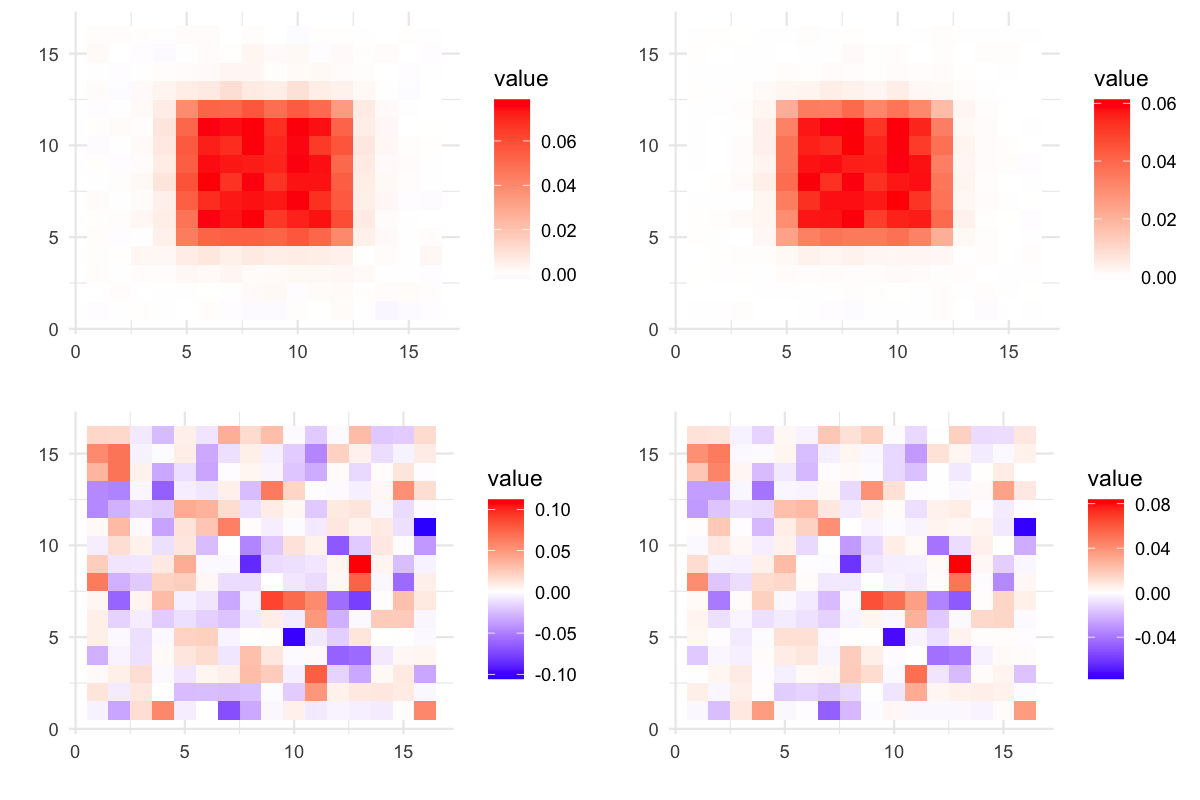
\includegraphics[width=0.8\textwidth]{beta_estimates.png}
	\caption{Mean estimated \( \beta \) values across simulations, with models fitted using \texttt{lambda.min} (left) and
		\texttt{lambda.1se} (right). The top row shows results for Simulation 1, while the bottom row shows results for Simulation 2.}
	\label{fig:beta_estimates}
\end{figure}

\begin{figure}[h!]
	\centering
	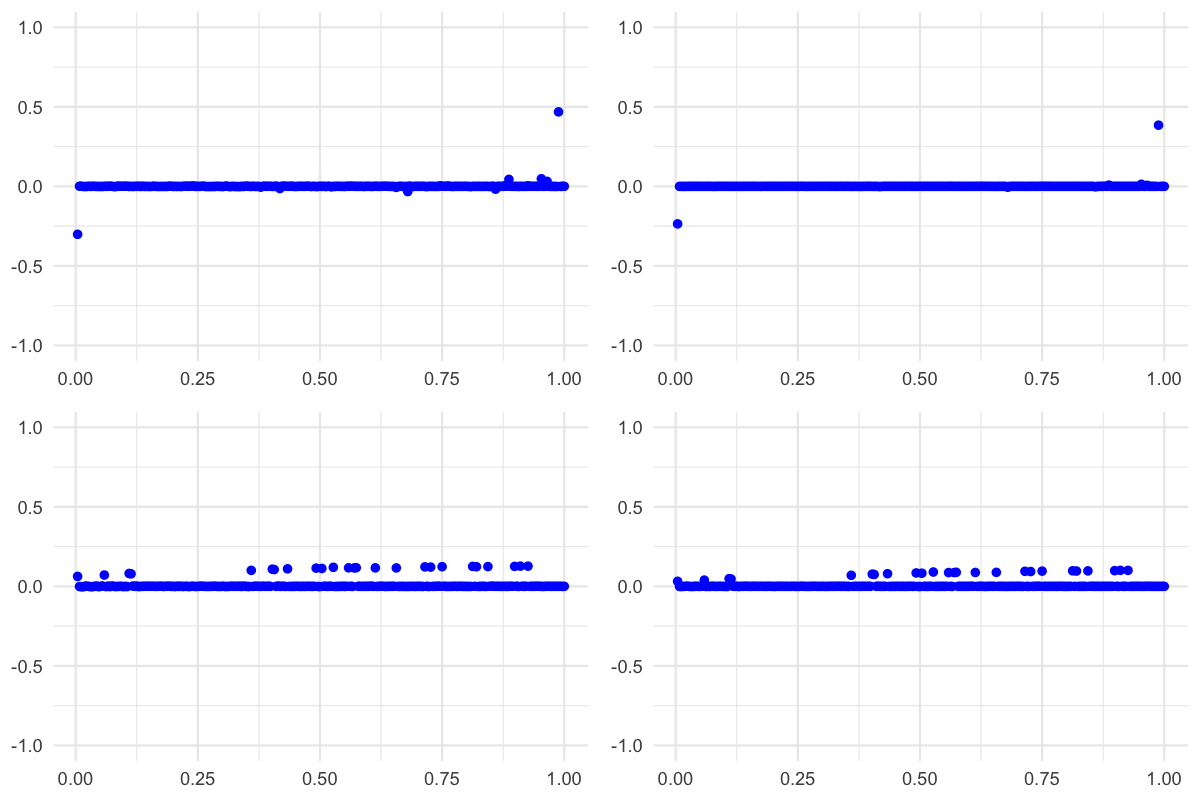
\includegraphics[width=0.8\textwidth]{b_estimates.png}
	\caption{Mean estimated \( b \) values across simulations, plotted against ordered eigenvalues. Models fitted using
		\texttt{lambda.min} are on the left and models fitted with \texttt{lambda.1se} on the right. The top row shows results for Simulation 1, while the bottom row shows results for Simulation 2.}
	\label{fig:b_estimates}
\end{figure}

\FloatBarrier

\subsection*{Significant P-values}

It is interesting to observe that, although the heatmap for significance of \( \beta \) in Simulation 1 follows the pattern of the actual non-zero values, the percentage of significance is relatively low (Figure \ref{fig:perc_sign_beta} left). In contrast, the non-zero values of \( \mathbf{b} \) (Figure \ref{fig:perc_sign_b} left) show a much higher percentage of significance, reaching as high as 100\% across iterations.

Another observation is that, although the non-zero effect size for \( \mathbf{b} \) is constant in Simulation 2, the percentage of significant p-values increases as the eigenvalues grow (Figure \ref{fig:perc_sign_b} right). [I am considering creating a plot to visualize the actual \( \beta \) values in Simulation 2 and the actual \( b \) values in Simulation 1, where the non-zero values vary, and compare them with the corresponding percentage of significant p-values. The goal is to examine whether the size of the actual non-zero values correlates with the percentage of significance. I suspect that a larger absolute effect size should result in a higher percentage of significance, but this doesn’t seem to be the case for \( b \) in Simulation 2, so I want to investigate other factors as well.]

\begin{figure}[h!]
	\centering
	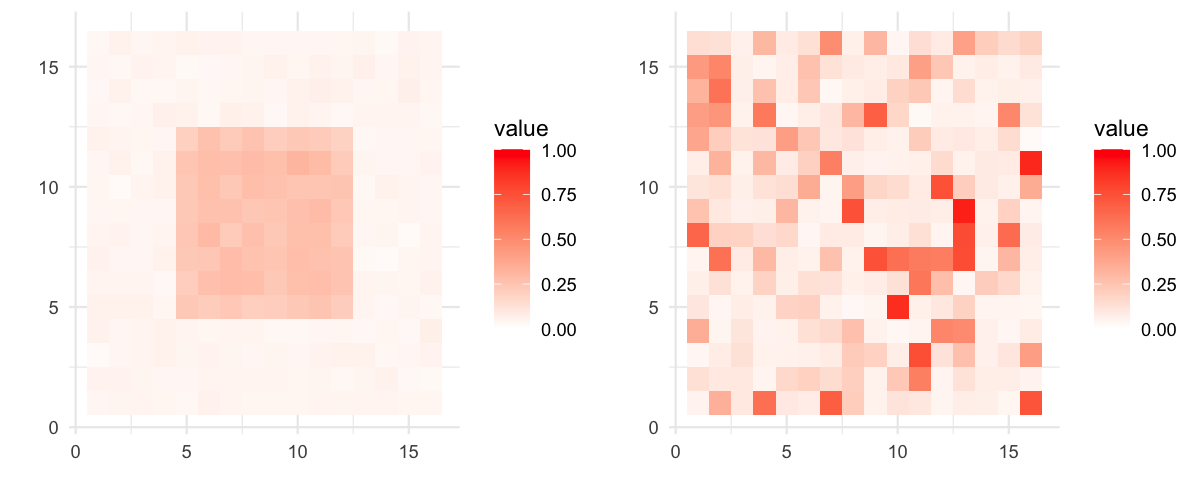
\includegraphics[width=0.9\textwidth]{perc_sign_pvals_hdi_beta.png}
	\caption{Percentage of significant p-values for elements of \( \beta \) when fitting models in the pixel space in
		Simulation 1 (left) and Simulation 2 (right).}
	\label{fig:perc_sign_beta}
\end{figure}

\begin{figure}[h!]
	\centering
	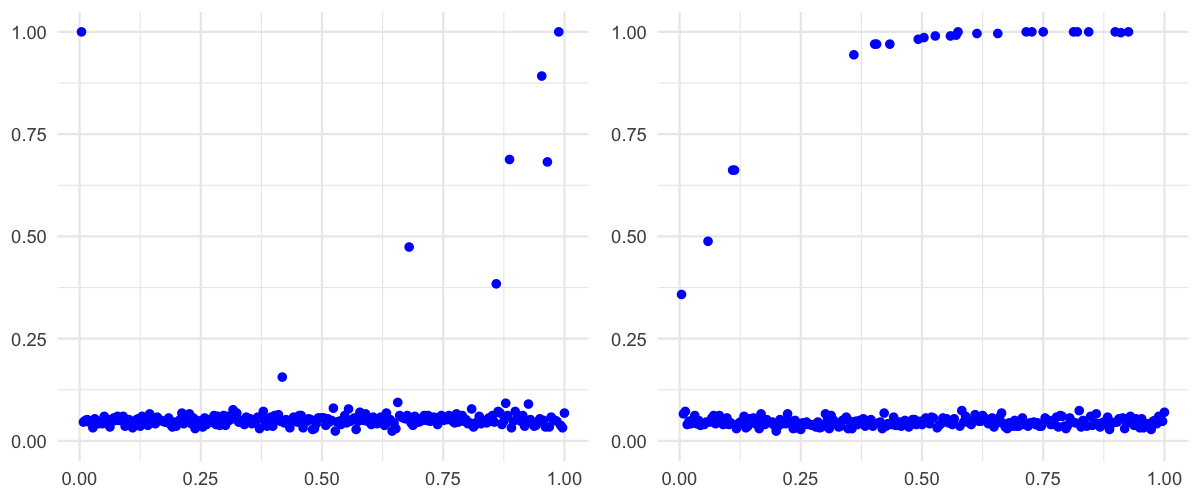
\includegraphics[width=0.9\textwidth]{perc_sign_pvals_hdi_b.png}
	\caption{Percentage of significant p-values for elements of \( b \) across ordered eigenvalues in both simulations.}
	\label{fig:perc_sign_b}
\end{figure}

\FloatBarrier


\section*{Future Work}

\begin{itemize}
  \item Adding details about how \texttt{hdi} package calculated p-values and why my permutation test didn't work.
  \item Increase \( b \) effect size (how to keep \( p \) evenly distributed in the same time?) see whether the pattern of coefficient estimates disappear or relieve.
  \item What is the next step in higher level?
\end{itemize}

\footnotesize
\bibliographystyle{abbrv}
\bibliography{references}

\end{document}


